% !TeX spellcheck = en_US

\chapter{Example Integration of new Module}\label{chap:add}
This chapter shows the extensibility of the framework by adding a new $aptitude$ package manager module for the Bash language. %\\
Section~\ref{sec:aptitude} provides common information about $aptitude$. %\\
In section~\ref{sec:aptitude_imp} the module is developed and integrated into the Bash language module.

\section{Aptitude Package Manager}\label{sec:aptitude}
This section describes the $aptitude$ package manager.
Like to $apt$-$get$, $aptitude$ is a command line program, where a package can be installed using the $aptitude$ $install$ \emph{package} command. 
In additional, it can be started in a pseudo-graphical mode to provide a visual interface shown in Figure~\ref{fig:aptitude_gui}).
An another advantage compared to $apt$-$get$ is the capability to search for packages by a part of the name (or by any other attributes) using the $aptitude$ $search$ $text$ command.
\begin{figure}[ht]   
	\centering
	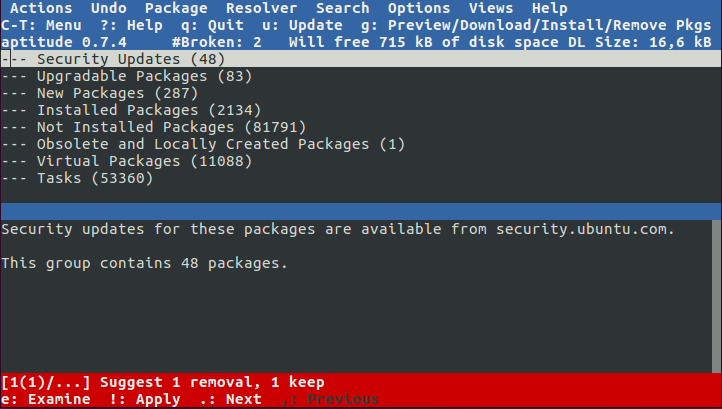
\includegraphics[width=0.7\textwidth]{Screenshot_aptitude.png}
	\caption{The command line visual interface for the $aptitude$ package manager.}
	\label{fig:aptitude_gui}
\end{figure}

\section{Development of Aptitude Module}\label{sec:aptitude_imp}
The implementation of the $aptitude$ module will be described here.
At first, the $aptitude$ class will be inherited from the abstract class $PackageManager$. 
This is presented in listing~\ref{lst:aptit_inher}. %\\
After that, the $aptitude$ class can be used as a regular package manager module, but it lacking functionality.
It is necessary to add the common code, like the constructor and the manager's name.
After these operations, the $aptitude$ module can be presented in listing~\ref{lst:aptit_common}. %\\
\begin{Listing} 
	\caption{The $aptitude$ module inherited from the $PackageManager$ abstract class}
	\label{lst:aptit_inher}
\begin{lstlisting}
public final class PM_aptitude extends PackageManager {
	@Override
	public List<String> proceed(String filename, String source)
		throws FileNotFoundException, IOException, JAXBException {
		// TODO Auto-generated method stub
	}
}
\end{lstlisting}
\end{Listing} 
\begin{Listing} 
\caption{The $aptitude$ module with some common elements}
\label{lst:aptit_common}
\begin{lstlisting}
public final class PM_aptitude extends PackageManager {

	// name of the package manager
	static public final String Name = "aptitude";
	
	/**
	* Constructor
	*/
	public PM_aptitude(Language language, CSAR_handler ch) {
		this.language = language;
		this.ch = ch;
	}
	
	@Override
	public List<String> proceed(String filename, String source)
		throws FileNotFoundException, IOException, JAXBException {
		// TODO Auto-generated method stub
	}
}
\end{lstlisting}
\end{Listing} 
Since the package manager will read files from an input CSAR, the CSAR handler is stored by the constructor to the $ch$ variable for a further use.
In addition, a pointer to the language (to Bash in this case) is stored too, to be propagated later to the package handler.\\
Now consider the $proceed$ function.
A line-by-line file analyzer is needed.
It must modify the data and in the case of changes, the $isChanged$ variable should be set to $true$.
The $isChanged$ variable indicates that the file must be rewritten with a new content from the $newFile$ variable.
In the $output$ variable a set of packages from the package handler will be stored and returned back to the Bash module.
Described behavior is implemented in listing~\ref{lst:aptit_proceed}.\\
An $aptitude$ line parser will be implemented.
It must read a line from the $line$ variable and store it or it's modified version into the $newFile$ variable.
If the data was changed, then the $isChanged$ variable must be set to $true$.
Any $aptitude$ package installation calls should be detected, commented out and its arguments (package names) should be propagated one by one to the package handler's function $getPackage$. 
The result of the $getPackage$ function will be added to the $output$ variable.\\
During the parsing which is defined in the listing \ref{lst:aptit_parse}, the line is divided into words. 
Each found package name is transmitted to the packet handler as an argument of its public function $getPackage$.
In additional, this function must take the language and the source artifact's name as the arguments.
\begin{Listing} 
\caption{The $aptitude$ module $proceed$ function}
\label{lst:aptit_proceed}
\begin{lstlisting}
@Override
public void proceed(String filename, String source)
	throws FileNotFoundException, IOException, JAXBException {
	if (ch == null)
		throw new NullPointerException();
	List<String> output = new LinkedList<String>();
	System.out.println(Name + " proceed " + filename);
	BufferedReader br = new BufferedReader(new FileReader(filename));
	boolean isChanged = false;
	String line = null;
	String newFile = "";
	while ((line = br.readLine()) != null) {
		// TODO parsing will be done here
	}
	br.close();
	if (isChanged)
		Utils.createFile(filename,newFile);
	return output;
}	 
\end{lstlisting}
\end{Listing} 
\begin{Listing} 
\caption{The $aptitude$ module line parser}
\label{lst:aptit_parse}
\begin{lstlisting}
String[] words = line.replaceAll("[;&]", "").split("\\s+");
// skip spaces at the beginning of string
int i = 0;
if (words[i].equals(""))
	i = 1;
// looking for aptitude 
if (words.length >= 1 + i && words[i].equals("aptitude")) {
	// aptitude found
	if (words.length >= 3 + i && words[1 + i].equals("install")) {
		System.out.println("aptitude found:" + line);
		isChanged = true;
		for (int packet = 2 + i; packet < words.length; packet++) {
			System.out.println("package: " + words[packet]);
			output.addAll(ch.getPackage(language, words[packet], source));
		}
	}
	newFile += "#//References resolver//" + line + '\n';
} 
else
	newFile += line + '\n';
\end{lstlisting}
\end{Listing} 
%\subsection*{Integration Aptitude into the Bash Module}\label{sec:aptitude_int}
\\
Now the $aptitude$ module can be added to the Bash module.
The only thing to do is to add the $aptitude$ to the Bash's list of package manager modules (the list is stored in the \emph{packageManagers} variable).
This is done by the Bash's constructor with the command: \emph{"packageManagers.add(new PM\_aptitude(this, ch));"}. %\\
After these operation the new module is ready to identify and resolve external references which use the $aptitude$ package manager to install packages.